%!\subsection{Future Trends and speculations}
%!\label{subsec:Futuretrends}

%!==========================
%Speculate on the potential future trajectories of architectural design, digital fabrication, and mixed reality. Discuss how these trends might shape the built environment, and propose ideas for further research and exploration.
%!==========================

%!\subsection{Object-Oriented Ontology}
%!\label{subsec:ObjectOrientedOntology}
% add the concept of Object-Oriented. Using these concepts as basis. I want to express that the mr experiment is based on the idea that architecture as a tool should be invisible and confortable while in use. But it should  create emotion when seen as part of the landscape as a form of art to recapture the humand oriented city .


It may be cheaper and quicker to build a load-bearing brick wall, but
the High Tech architect will always prefer the steel frame and the lightweight metal panel because this is a technique more in tune with the spirit of the age.
He is committed to the idea that building must eventually catch up with the rest of technology, and he is determined to "drag building into the twentieth century".\cite{Davies1988}

Contemporary avant-garde architecture is addressing the demand for an increased level of
articulated complexity by means of retooling its methods on the basis of parametric design
systems.\cite{Schumacher2008}

The concept of style must therefore be sharply distinguished and cleansed of these
trivialising and distracting connotations.
It denotes the unity of the difference between the architectural epochs of gothic, renaissance, baroque, classicism, historicism and modernism.The historical self-consciousness of architecture demands the revitalisation of the concept of style as a profound historical phenomenon that can be projected into the future.\cite{Schumacher2010}


For this purpose I have proposed that architectural styles are best understood as design-research programmes, conceived in analogy to the way paradigms frame scientific research programmes. \cite{Schumacher2010}

%! important quote about styles
Innovation in architecture proceeds via the progression of styles so understood.
This implies the alternation between periods of cumulative advancement within a style, and revolutionary periods of transition between styles.
Styles represent long, sustained cycles of innovation, gathering design-research efforts into a collective movement so that individual efforts are mutually relevant,spurning and enhancing.\cite{Schumacher2010}


This is the idea of a unified style;
initially as a unified avant-garde design-research programme, and eventually as a unified system of principles, ambitions and values that constitute global best practice.\cite{Schumacher2010}


parametricism can take up vernacular, classical, modernist, post-modernist, deconstructivist and minimalist urban conditions, and forge a new network of affiliations and continuities between and beyond any number of urban fragments and conditions. \cite{Schumacher2010}


There has been talk about versioning, iteration and mass customization, etc., for quite a while within the architectural avant-garde discourse. \cite{Schumacher2008}


Modernism’s crisis and its architectural aftermath has led many critics to believe we can no longer be expected to forge a unified style.\cite{Schumacher2010}


Heideggers tool analysis states that as the tool is a tool it disappears in favor of some purpose he continues to explain that generally we don't notice equipment until it fails, like when An earthquake calls attention to the ground we walk or when a medical problem alerts us of the presence of organs that we have silently depended\cite{Harman2011}.

Harmans, Object-oriented ontology, borrows this concept to formulate its central claim that objects have hidden qualities and realities, and they withdraw from our understanding.\cite{Gage2015}
he idea that we live our lives on a layer of invisible equipment has significant ramifications for architecture, a discipline that produces the equipment on and in which we exist.\cite{Gage2015}

(Figure \ref{fig:complexornament})

%% Figure of Contemporary timeline
     \begin{figure*}[htb]
          \centering
          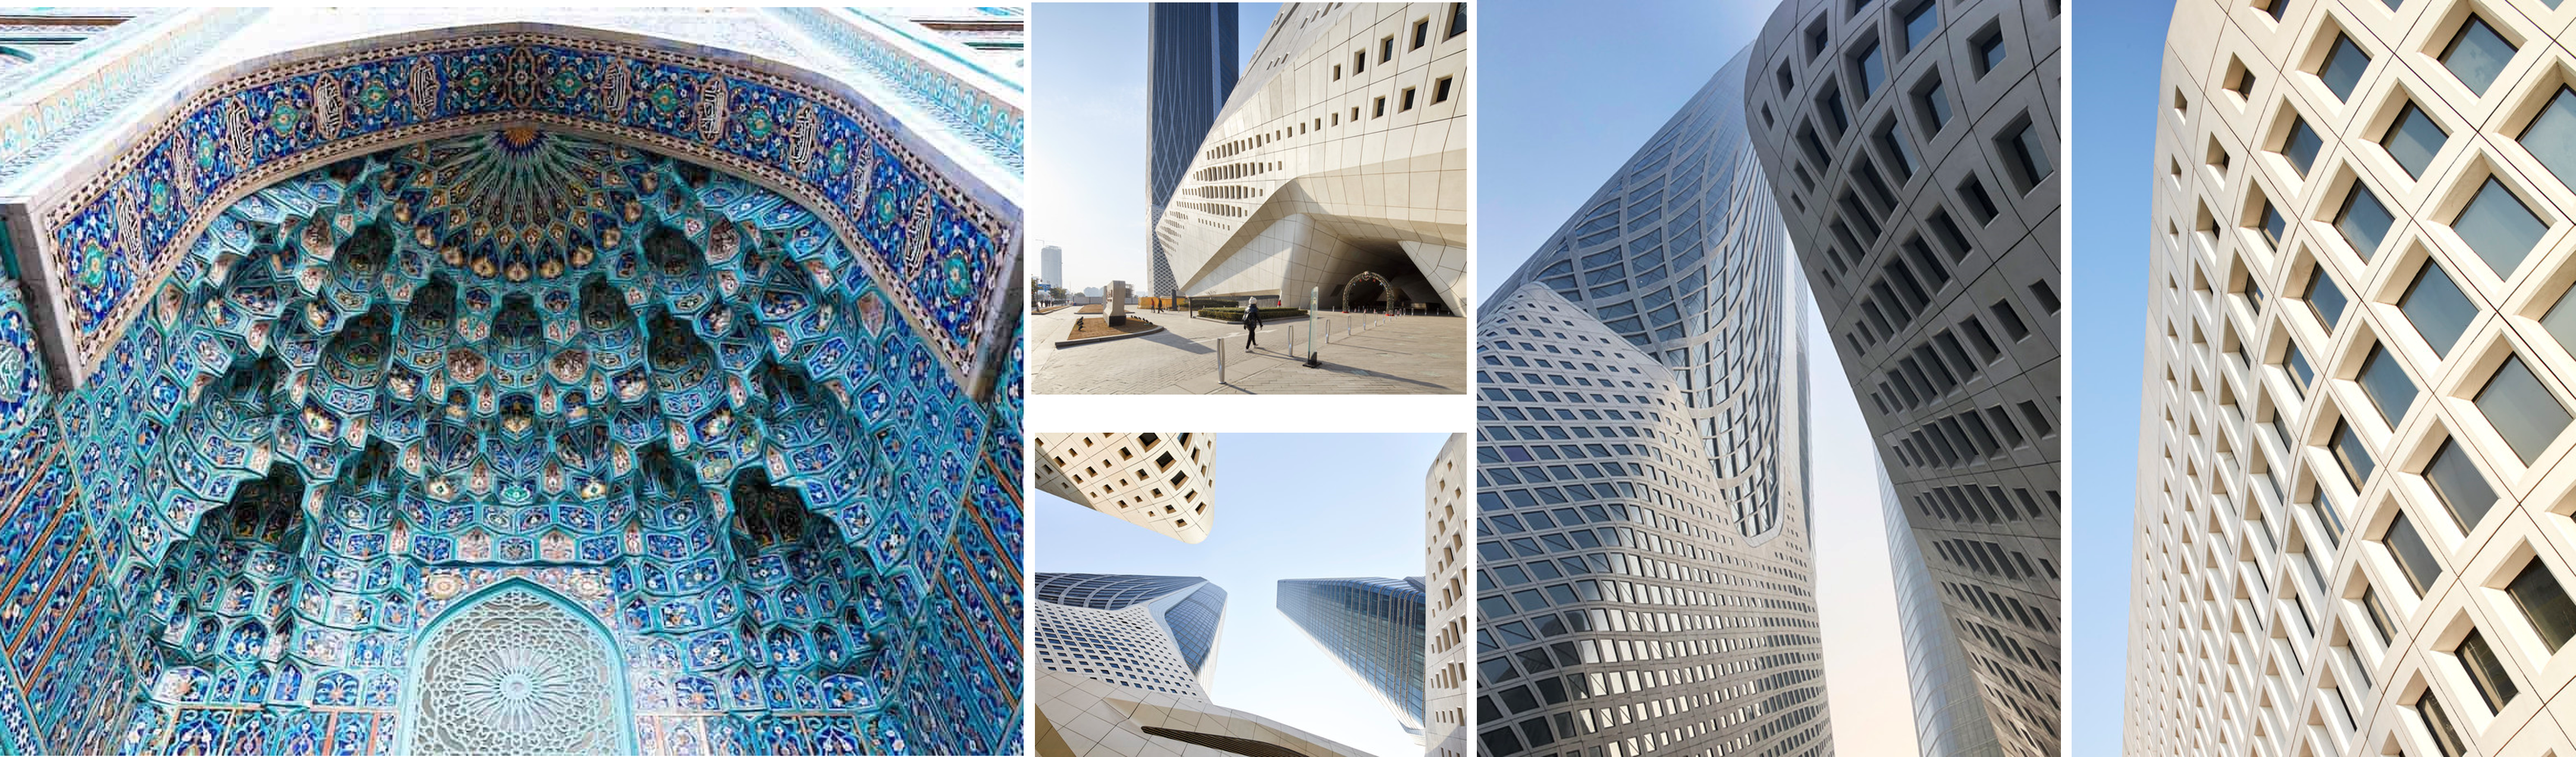
\includegraphics[width= \linewidth]{Images/complexornament}
          \caption{Complex ornament reference  (\textit{Images edited from source)}}
          \label{fig:complexornament}
        \end{figure*}
